% Options for packages loaded elsewhere
\PassOptionsToPackage{unicode}{hyperref}
\PassOptionsToPackage{hyphens}{url}
%
\documentclass[
]{article}
\title{iButton Temperature Data from 40 Aquatic Plots}
\author{Emily Watson-Cook, Jana Peirce}
\date{19 February 2022}

\usepackage{amsmath,amssymb}
\usepackage{lmodern}
\usepackage{iftex}
\ifPDFTeX
  \usepackage[T1]{fontenc}
  \usepackage[utf8]{inputenc}
  \usepackage{textcomp} % provide euro and other symbols
\else % if luatex or xetex
  \usepackage{unicode-math}
  \defaultfontfeatures{Scale=MatchLowercase}
  \defaultfontfeatures[\rmfamily]{Ligatures=TeX,Scale=1}
\fi
% Use upquote if available, for straight quotes in verbatim environments
\IfFileExists{upquote.sty}{\usepackage{upquote}}{}
\IfFileExists{microtype.sty}{% use microtype if available
  \usepackage[]{microtype}
  \UseMicrotypeSet[protrusion]{basicmath} % disable protrusion for tt fonts
}{}
\makeatletter
\@ifundefined{KOMAClassName}{% if non-KOMA class
  \IfFileExists{parskip.sty}{%
    \usepackage{parskip}
  }{% else
    \setlength{\parindent}{0pt}
    \setlength{\parskip}{6pt plus 2pt minus 1pt}}
}{% if KOMA class
  \KOMAoptions{parskip=half}}
\makeatother
\usepackage{xcolor}
\IfFileExists{xurl.sty}{\usepackage{xurl}}{} % add URL line breaks if available
\IfFileExists{bookmark.sty}{\usepackage{bookmark}}{\usepackage{hyperref}}
\hypersetup{
  pdftitle={iButton Temperature Data from 40 Aquatic Plots},
  pdfauthor={Emily Watson-Cook, Jana Peirce},
  hidelinks,
  pdfcreator={LaTeX via pandoc}}
\urlstyle{same} % disable monospaced font for URLs
\usepackage[margin=1in]{geometry}
\usepackage{longtable,booktabs,array}
\usepackage{calc} % for calculating minipage widths
% Correct order of tables after \paragraph or \subparagraph
\usepackage{etoolbox}
\makeatletter
\patchcmd\longtable{\par}{\if@noskipsec\mbox{}\fi\par}{}{}
\makeatother
% Allow footnotes in longtable head/foot
\IfFileExists{footnotehyper.sty}{\usepackage{footnotehyper}}{\usepackage{footnote}}
\makesavenoteenv{longtable}
\usepackage{graphicx}
\makeatletter
\def\maxwidth{\ifdim\Gin@nat@width>\linewidth\linewidth\else\Gin@nat@width\fi}
\def\maxheight{\ifdim\Gin@nat@height>\textheight\textheight\else\Gin@nat@height\fi}
\makeatother
% Scale images if necessary, so that they will not overflow the page
% margins by default, and it is still possible to overwrite the defaults
% using explicit options in \includegraphics[width, height, ...]{}
\setkeys{Gin}{width=\maxwidth,height=\maxheight,keepaspectratio}
% Set default figure placement to htbp
\makeatletter
\def\fps@figure{htbp}
\makeatother
\setlength{\emergencystretch}{3em} % prevent overfull lines
\providecommand{\tightlist}{%
  \setlength{\itemsep}{0pt}\setlength{\parskip}{0pt}}
\setcounter{secnumdepth}{-\maxdimen} % remove section numbering
\ifLuaTeX
  \usepackage{selnolig}  % disable illegal ligatures
\fi

\begin{document}
\maketitle

Thermocron iButton data loggers were installed on July 19, 2021, in 30
thaw ponds in the NIRPO and Jorgenson Field Sites, Prudhoe Bay, Alaska,
and programmed to record temperature in degrees Celsius every hour. They
were retrieved on August 23, 2021.

Sensors were installed in the following locations in each pond:

\begin{itemize}
\tightlist
\item
  Water surface
\item
  Above the moss layer
\item
  At the sediment surface.
\end{itemize}

Two additional sensors were installed to record air temperature at each
site (NIRPO and Jorgenson), and one sensor was installed at the water
surface in a lake at the Jorgenson site.

\hypertarget{raw-data-99720-rows}{%
\subsubsection{Raw Data (99,720 rows)}\label{raw-data-99720-rows}}

\begin{longtable}[]{@{}lllrlll@{}}
\toprule
Date & Time & iBtn ID & Temp (°C) & Plot ID & Sensor Type & Plot Type \\
\midrule
\endhead
2021-07-19 & 6:00:00 PM & 1 & 20.5 & 21A-01 & Aquatic forb & Water
surface \\
2021-07-19 & 6:00:00 PM & 2 & 20.5 & 21A-01 & Aquatic forb & Above
moss \\
2021-07-19 & 6:00:00 PM & 4 & 13.0 & 21A-01 & Aquatic forb & Sediment \\
2021-07-19 & 6:00:00 PM & 5 & 21.5 & 21A-02 & Thick moss & Water
surface \\
2021-07-19 & 6:00:00 PM & 6 & 21.5 & 21A-02 & Thick moss & Above moss \\
2021-07-19 & 6:00:00 PM & 9 & 8.5 & 21A-02 & Thick moss & Sediment \\
\bottomrule
\end{longtable}

\hypertarget{average-daily-temperature-calculated-4320-rows}{%
\subsubsection{Average Daily Temperature calculated (4320
rows)}\label{average-daily-temperature-calculated-4320-rows}}

\begin{longtable}[]{@{}lllllr@{}}
\toprule
Date & iBtn ID & Plot ID & Sensor Type & Plot Type & Avg Daily Temp
(°C) \\
\midrule
\endhead
2021-07-19 & 1 & 21A-01 & Water surface & Aquatic forb & 20.1 \\
2021-07-19 & 10 & 21A-03 & Sediment & Aquatic forb & 8.8 \\
2021-07-19 & 101 & 21A-20 & Sediment & Lake & 15.7 \\
2021-07-19 & 103 & 21A-21 & Water surface & Thick moss & 20.5 \\
2021-07-19 & 105 & 21A-21 & Above moss & Thick moss & 20.8 \\
2021-07-19 & 108 & 21A-21 & Sediment & Thick moss & 7.2 \\
\bottomrule
\end{longtable}

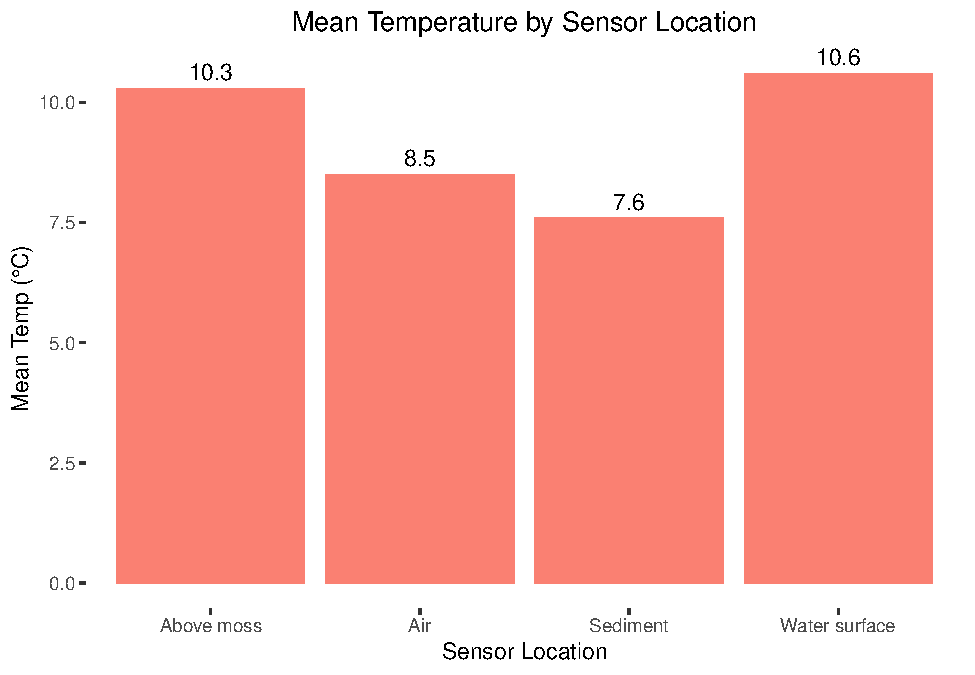
\includegraphics{iButtons-aquatic-veg-NIRPO-JS-2021_files/figure-latex/unnamed-chunk-11-1.pdf}

\begin{longtable}[]{@{}lr@{}}
\toprule
Sensor Type & Mean Temp (°C) \\
\midrule
\endhead
Above moss & 10.3 \\
Air & 8.5 \\
Sediment & 7.6 \\
Water surface & 10.6 \\
\bottomrule
\end{longtable}

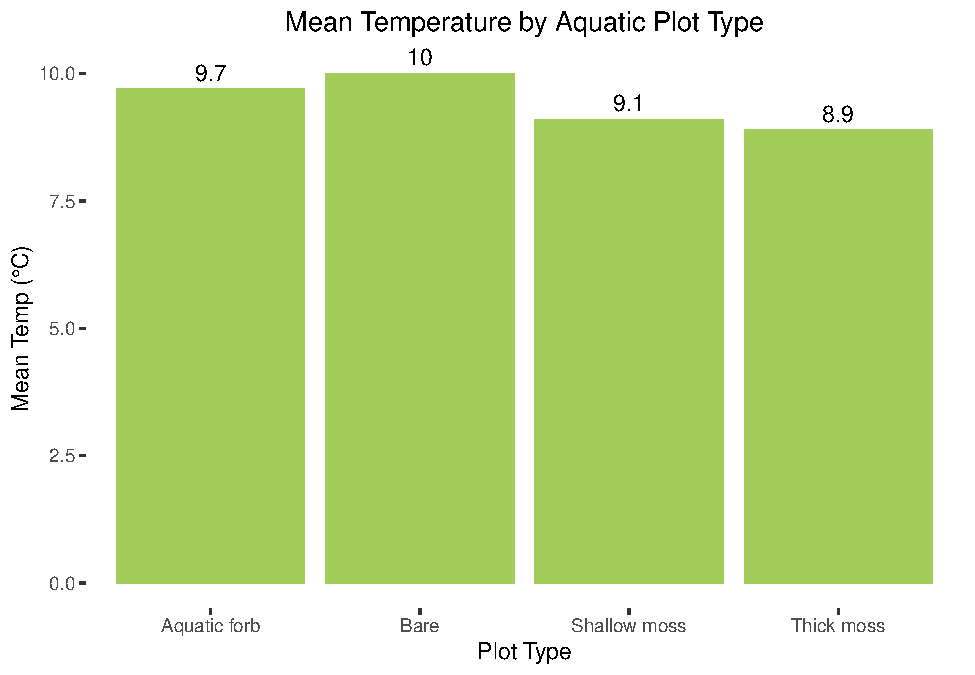
\includegraphics{iButtons-aquatic-veg-NIRPO-JS-2021_files/figure-latex/unnamed-chunk-14-1.pdf}

\begin{longtable}[]{@{}lr@{}}
\toprule
Plot Type & Mean Temp (°C) \\
\midrule
\endhead
Aquatic forb & 9.7 \\
Bare & 10.0 \\
Shallow moss & 9.1 \\
Thick moss & 8.9 \\
\bottomrule
\end{longtable}

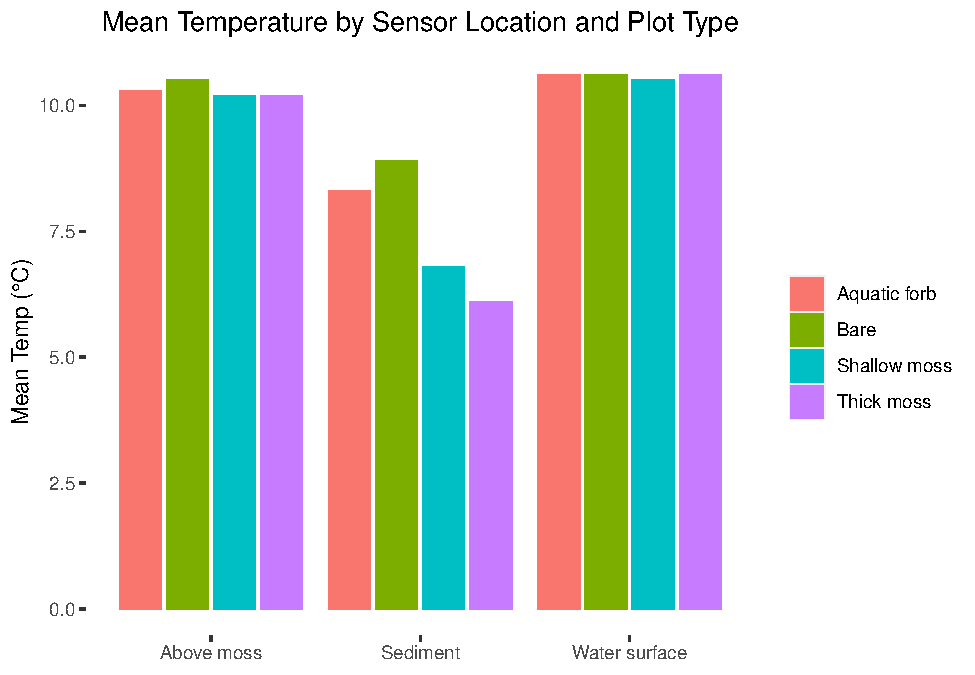
\includegraphics{iButtons-aquatic-veg-NIRPO-JS-2021_files/figure-latex/unnamed-chunk-15-1.pdf}

\begin{longtable}[]{@{}llr@{}}
\toprule
Sensor Type & Plot Type & Mean Temp (°C) \\
\midrule
\endhead
Above moss & Aquatic forb & 10.3 \\
Above moss & Bare & 10.5 \\
Above moss & Shallow moss & 10.2 \\
Above moss & Thick moss & 10.2 \\
Sediment & Aquatic forb & 8.3 \\
Sediment & Bare & 8.9 \\
Sediment & Shallow moss & 6.8 \\
Sediment & Thick moss & 6.1 \\
Water surface & Aquatic forb & 10.6 \\
Water surface & Bare & 10.6 \\
Water surface & Shallow moss & 10.5 \\
Water surface & Thick moss & 10.6 \\
\bottomrule
\end{longtable}

\hypertarget{lets-look-at-the-data-in-more-detail.}{%
\subsubsection{Let's look at the data in more
detail.}\label{lets-look-at-the-data-in-more-detail.}}

Here is a plot of the average daily temperature of each iButton from
July 19 to August 23.

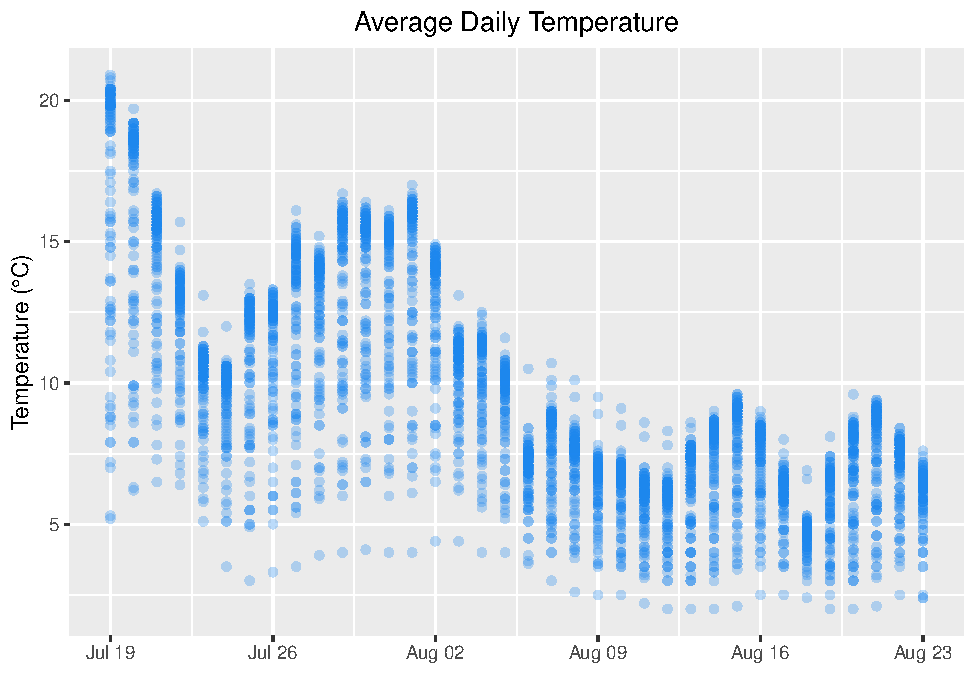
\includegraphics{iButtons-aquatic-veg-NIRPO-JS-2021_files/figure-latex/unnamed-chunk-16-1.pdf}
Now we can look at the same data but colored to indicated the location
of the temperature sensor: At water surface, sediment surface, or below
the water surface, but above the vegetation layer. Two sensors were also
placed above the ground to record the ambient air temperature at each
site.

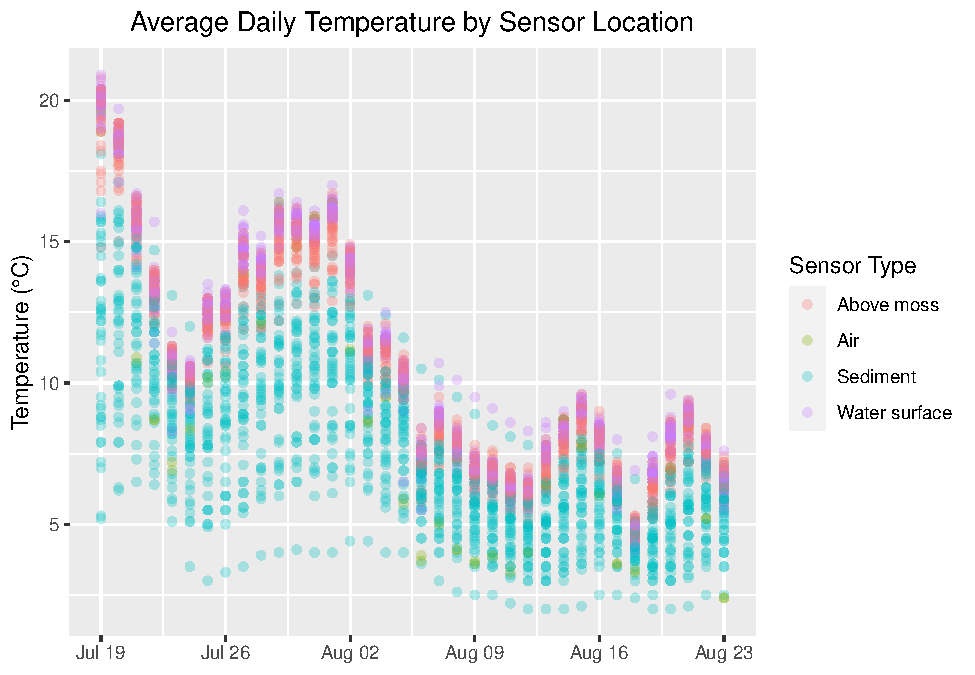
\includegraphics{iButtons-aquatic-veg-NIRPO-JS-2021_files/figure-latex/unnamed-chunk-17-1.pdf}
This time we'll look at the dominant type of aquatic vegetation in the
1-m plot. For example, here the plot shows the average daily temperature
data for each sensor location (water surface, sediment surface, above
moss layer) in thick moss plots as purple markers. Based onthe previous
plot we can assume the coldest temperatures in thick moss plots come
from the sensors at the sediment surface, and the warmest temperatures
are from the water surface.

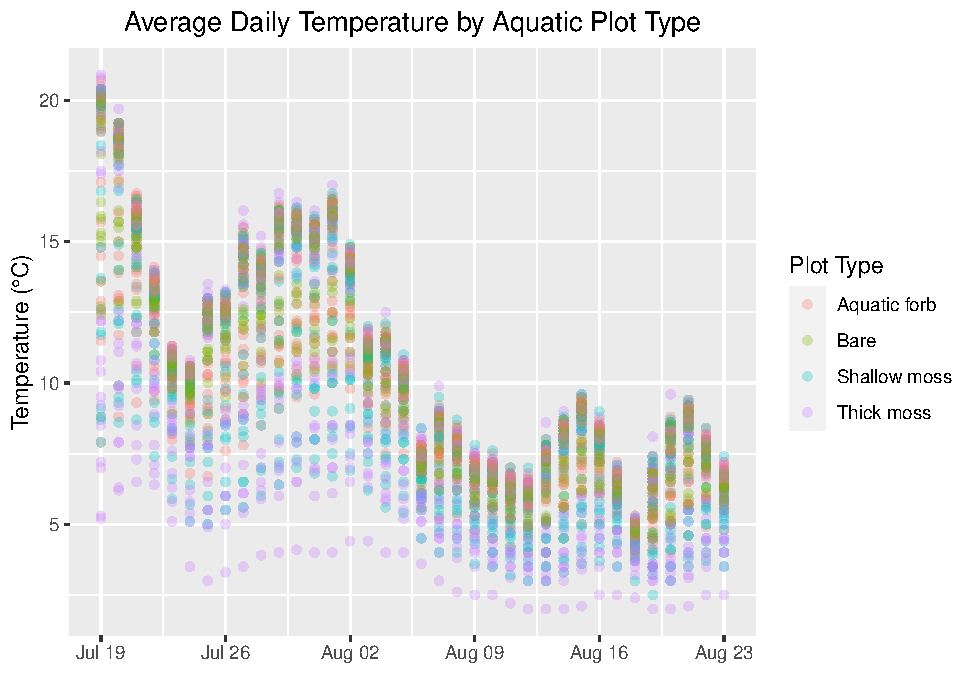
\includegraphics{iButtons-aquatic-veg-NIRPO-JS-2021_files/figure-latex/unnamed-chunk-19-1.pdf}

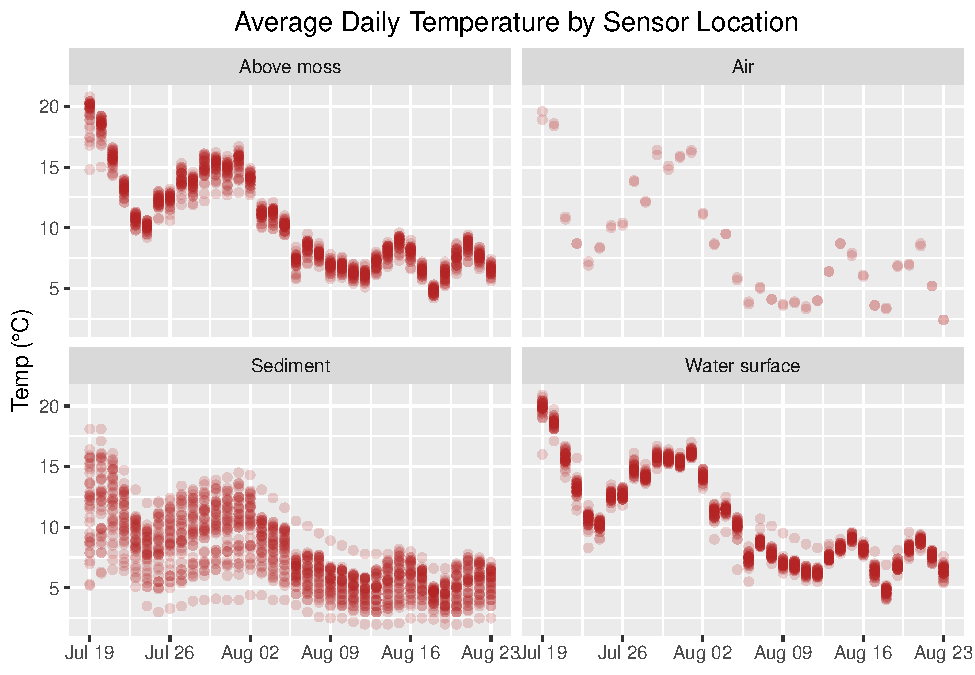
\includegraphics{iButtons-aquatic-veg-NIRPO-JS-2021_files/figure-latex/unnamed-chunk-20-1.pdf}

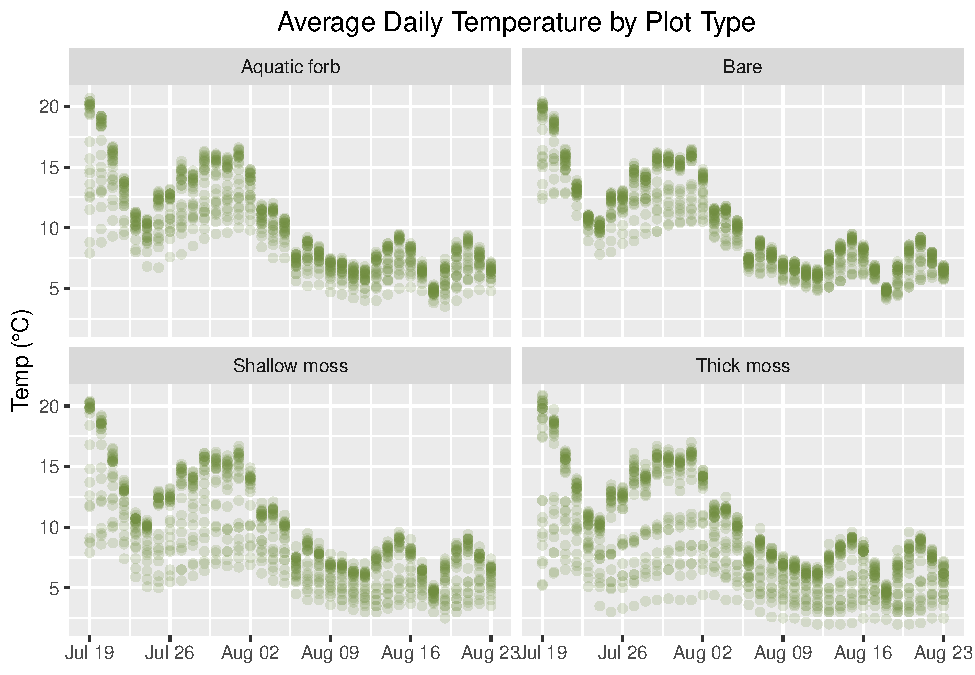
\includegraphics{iButtons-aquatic-veg-NIRPO-JS-2021_files/figure-latex/unnamed-chunk-21-1.pdf}

\hypertarget{whats-going-on-at-the-sediment-surface}{%
\subsubsection{What's going on at the sediment
surface?}\label{whats-going-on-at-the-sediment-surface}}

Let's take a closer look at the differences in temperature at the
sediment surface by plot type. As we've seen the coldest temperatures
are at the pond bottoms are in plots characterized by thick moss.

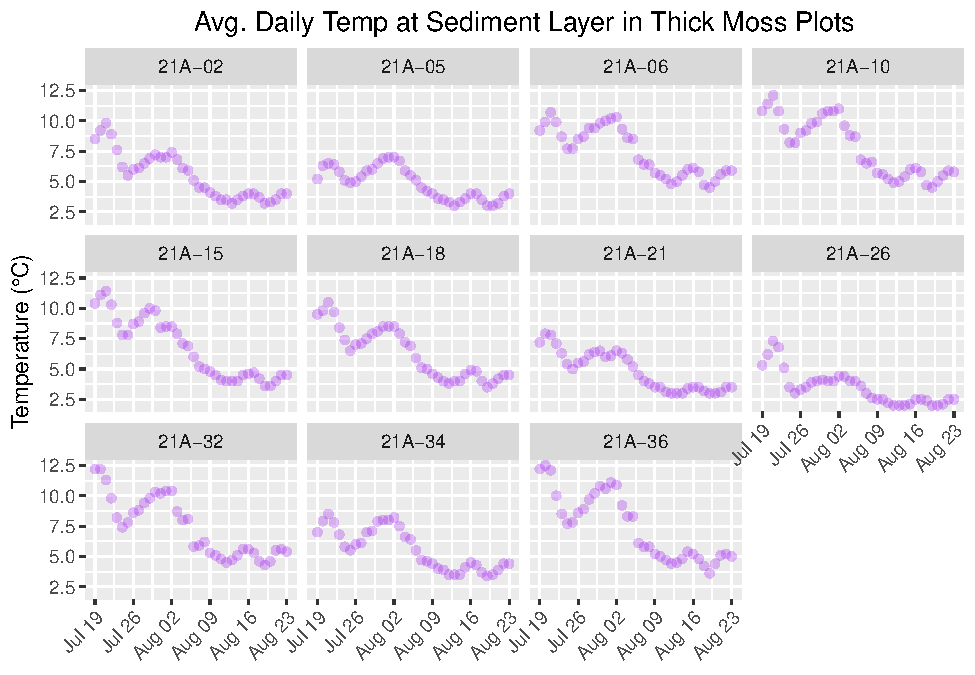
\includegraphics{iButtons-aquatic-veg-NIRPO-JS-2021_files/figure-latex/unnamed-chunk-23-1.pdf}

Followed by shallow moss\ldots{}

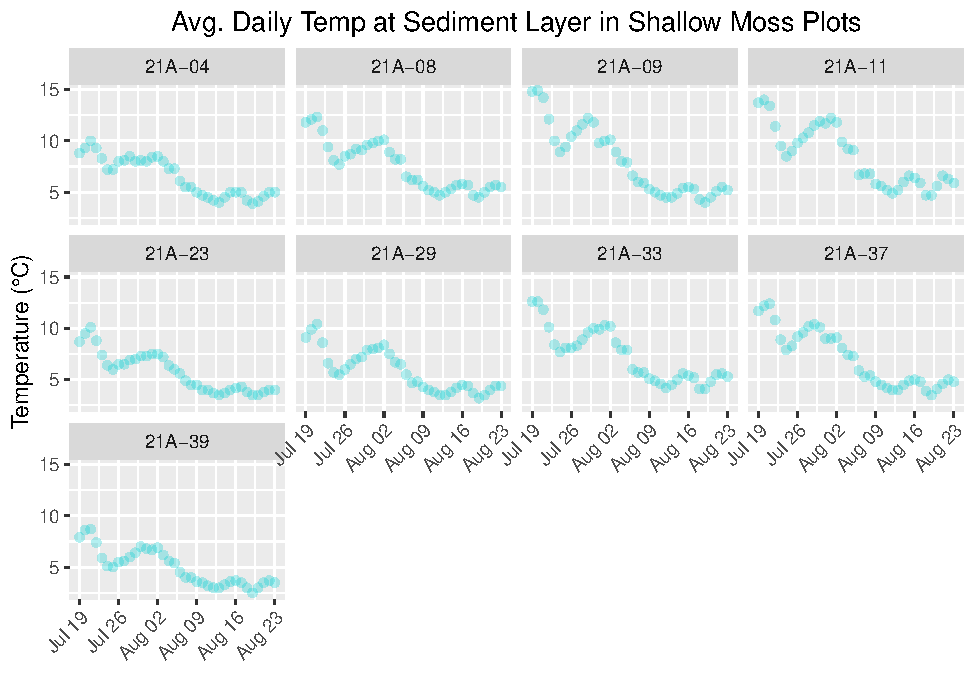
\includegraphics{iButtons-aquatic-veg-NIRPO-JS-2021_files/figure-latex/unnamed-chunk-25-1.pdf}
And aquatic forb plots\ldots{}

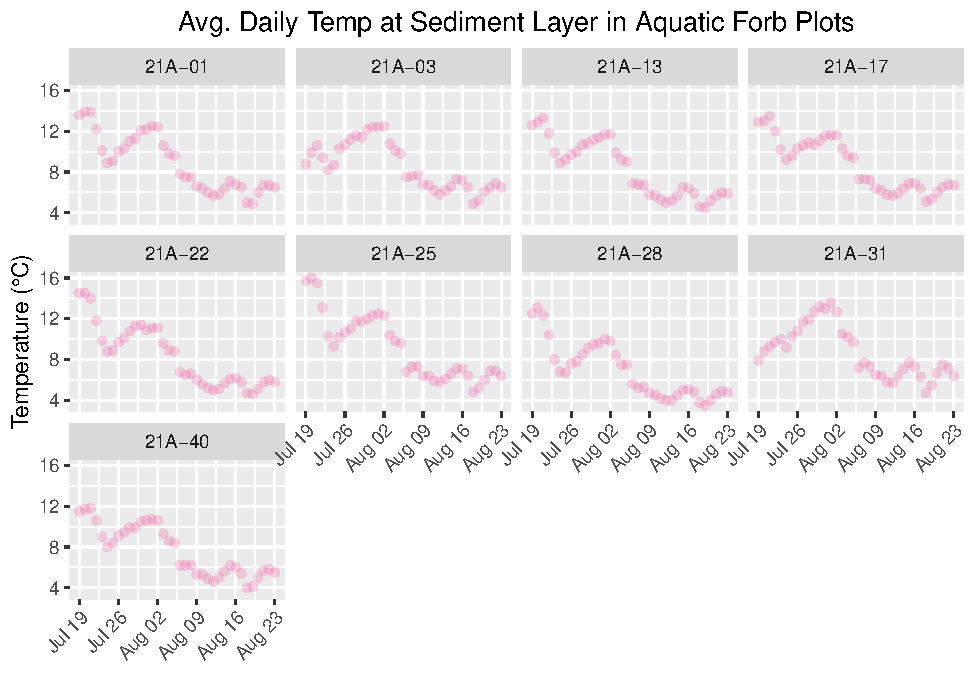
\includegraphics{iButtons-aquatic-veg-NIRPO-JS-2021_files/figure-latex/unnamed-chunk-27-1.pdf}

Finally, we observe the warmest temperatures at the pond bottom
(sediment surface location) in plots without significant vegetation of
any type (bare plots).

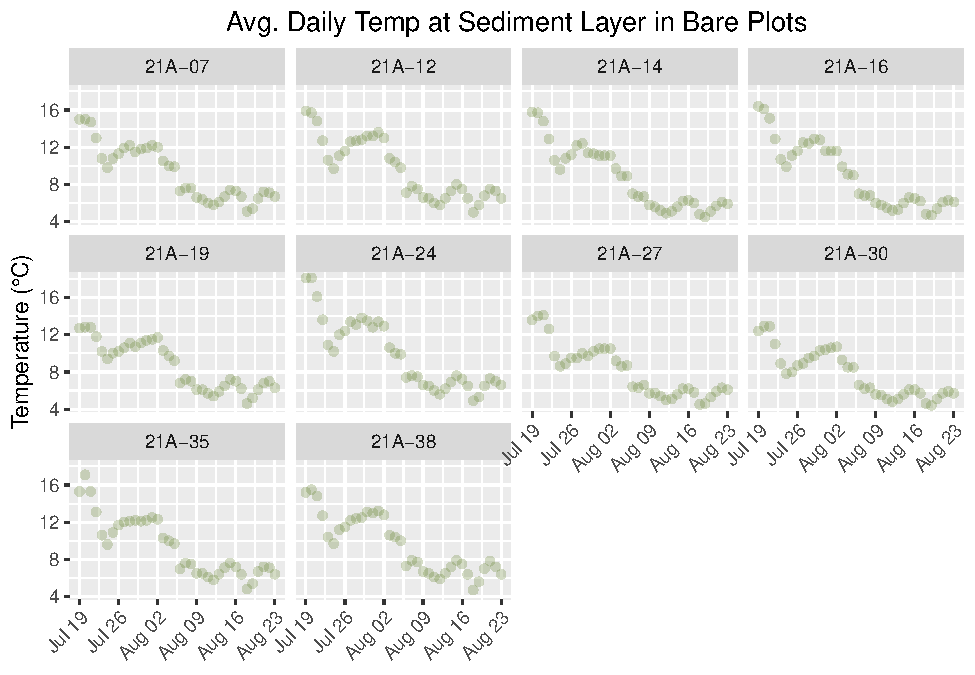
\includegraphics{iButtons-aquatic-veg-NIRPO-JS-2021_files/figure-latex/unnamed-chunk-29-1.pdf}

\end{document}
